\documentclass[10pt,a4paper]{report}
\usepackage[utf8]{inputenc}
\usepackage{amsmath}
\usepackage{amsfonts}
\usepackage{amssymb}
\usepackage{graphicx}
\usepackage{hyperref}
\usepackage{bm}
\usepackage{gensymb}
\usepackage[left=2cm,right=2cm,top=2cm,bottom=2cm]{geometry}
\setlength\parindent{0pt}
\graphicspath{{./images/}}
\begin{document}


\textbf{Additional Project 2.4: Simulation of Random Samples from Parametric Distributions}
\thispagestyle{empty}

\newpage

\subsection*{Question 1}

Given the pdf $f(x \hspace{1mm}| \hspace{1mm} \theta)$ is exponential, the median m satisfies:

\begin{align*}
\int_0^m f(x \hspace{1mm}| \hspace{1mm} \theta) dx &= \frac{1}{2}\\
\int_0^m \theta e^{-\theta x} dx &= \frac{1}{2}\\
\left[-e^{-\theta x}\right]_0^m &=\frac{1}{2}\\`
\theta &= \frac{\ln{2}}{m}
\end{align*}

Thus $g(x \hspace{1mm}| \hspace{1mm} m) = f(x \hspace{1mm}| \hspace{1mm} \theta(m)) = \frac{\ln2}{m}\exp(-\frac{\ln2}{m}x)$

\subsection*{Question 2}

Have 

\begin{align*}
l_n(m)&=\log\prod_{i=1}^ng(x \hspace{1mm}| \hspace{1mm} m)\\
&=\sum_{i=1}^n \ln(\ln2) - \ln m -\frac{\ln2}{m}x_i\\
&=n\ln(\ln 2)-n\ln m-\frac{\ln 2}{m}\sum x_i\\
\end{align*}

and thus 

\begin{align*}
\frac{\partial l_n(m)}{\partial m} &= 0\\
\Rightarrow \sum_{i=1}^n -\frac{1}{m} + \frac{ln2}{m}x_i &=0\\
\Rightarrow \hat{m_n} &= \frac{ln2\sum x_i}{n}=\frac{ln2}{\hat{\theta_n}}
\end{align*}

Now for $\theta_0=1.2$ we get the actual value of the median $m_0=\frac{ln2}{\theta_0}=0.5776$. Running the script $q2.m$ produced the output figure 1, and an $\hat{m_n}=0.4089$.

\begin{figure}[ht]
\centering
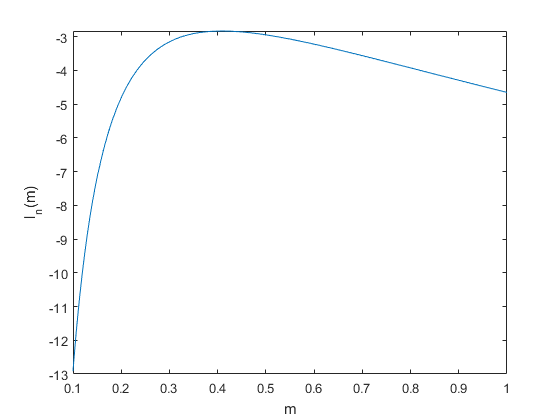
\includegraphics[width=0.5\textwidth]{q2n6.png}
\caption{A graph of $l_n(m)$ with n=6}
\end{figure}

\subsection*{Question 3}

\begin{figure}[ht]
\begin{minipage}[b]{0.5\linewidth}
\centering
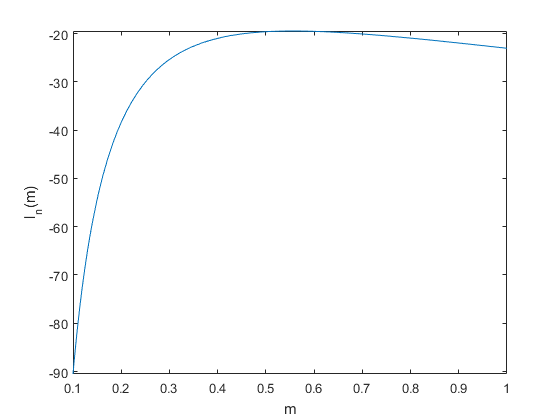
\includegraphics[width=\textwidth]{q3n25.png}
\caption{n=25 $\hat{m_n}=0.5557$}
\end{minipage}
\hspace{0.5cm}
\begin{minipage}[b]{0.5\linewidth}
\centering
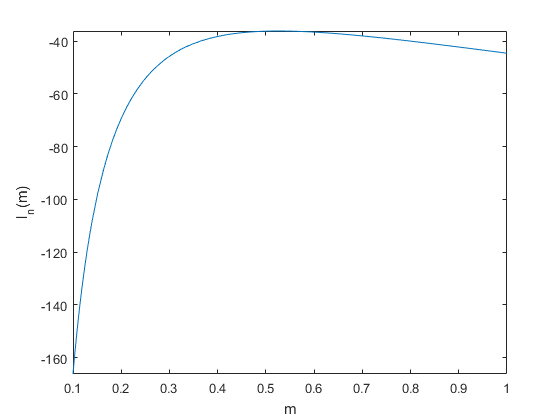
\includegraphics[width=\textwidth]{q3n50.png}
\caption{n=50 $\hat{m_n}=0.5260$}
\end{minipage}
\end{figure}


\begin{figure}[ht]
\centering
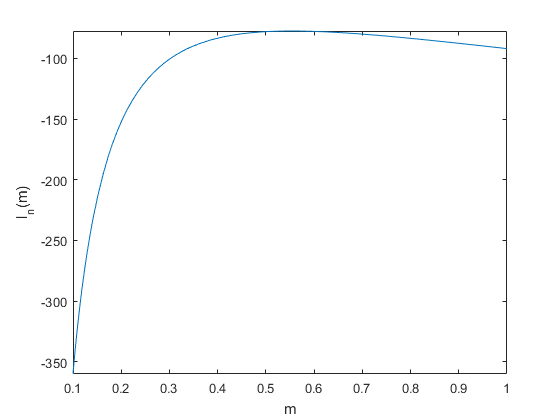
\includegraphics[width=0.5\textwidth]{q3n100.png}
\caption{n=100 $\hat{m_n}=0.5531$}
\end{figure}

We see little change in the shape of $l_n(m)$ as n is increased, since the functional form remains the same. Note that the coefficient $-\ln2\sum x_i$ has expectation $\frac{n\ln2}{1.2}$, thus $l_n(m)\approx n( \ln\ln 2-\ln m - \frac{ln2}{1.2m})$, so varying n doesn't change the shape. We do see the peak at $\hat{m_n}$ slowly approaches $m_0$ as n increases.

\subsection*{Question 4}

We have X,Y exponential with mean $\frac{1}{\theta}$ and thus are Exp($\theta$) with pdf $f(x)=\theta e^{-\theta x}$. Thus the moment generating function is

\begin{align*}
M_X(\lambda)&=\mathbb{E}[e^{\lambda X}]\\
&=\int_0^\infty \theta e^{x(\lambda - \theta)}dx\\
&=\frac{\theta}{\lambda-\theta}\left[-e^{x(\lambda-\theta)}\right]_0^\infty\\
&=\frac{\theta}{\theta-\lambda} \quad \text{for $\lambda<\theta$}
\end{align*}

Now to show $X+Y \sim \Gamma(2,\theta)$ note that

\begin{align*}
&M_{X+Y}(\lambda)\\
&=\mathbb{E}[e^{\lambda (X+Y)}]\\
&=\mathbb{E}[e^{\lambda X}e^{\lambda Y}]\\
&=\mathbb{E}[e^{\lambda X}]\mathbb{E}[e^{\lambda Y}] \quad \text{by independence of X and Y}\\
&=(\frac{\theta}{\theta-\lambda})^2\\
&=(1-\frac{\lambda}{\theta})^{-2} \quad \text{for $\lambda<\theta$}
\end{align*}

which is the moment generating function for a $\Gamma(2,\theta)$, and by uniqueness of moment generating functions, have  $X+Y \sim \Gamma(2,\theta)$.


\subsection*{Question 5}

Given the probability density function $f(x \hspace{1mm}| \hspace{1mm} \theta) = \theta^2xe^{-\theta x}$ we integrate it to find

\begin{align*}
F(x) &= \mathbb{P}(X \leq x)\\
	&= \int_0^x \theta^2ue^{-\theta u}du \\
	&= \left[-e^{-\theta x}(\theta x +1)\right]_0^x\\
	&= 1-e^{-\theta x}(\theta x +1)\\
\end{align*}

Note this pdf is of a $\Gamma(2,\theta)$ variable. F has no closed elementary inverse due to both $e^{-\theta x}$ and $xe^{-\theta x}$ terms.

\subsection*{Question 6}

Have 

\begin{align*}
l_n(\theta)&= \log\prod_{i=1}^n f(x_i \hspace{1mm}| \hspace{1mm} \theta)\\
&=\ln\prod_{i=1}^n \theta^2x_i e^{-\theta x_i}\\
&=\sum_{i=1}^n 2\ln \theta +\ln x_i -\theta x_i
\end{align*}

and thus 

\begin{align*}
\frac{\partial l_n(\theta)}{\partial \theta} &= 0\\
\Rightarrow \sum_{i=1}^n \frac{2}{\theta} - x_i &=0\\
\Rightarrow \hat{\theta_n} &= \frac{2n}{\sum x_i}
\end{align*}

\newpage

\subsection*{Question 7}
Despite not being able to invert F to generate a sample from f, we note from Question 4, to sample from f it suffices to sum two values taken from an Exp(2.2) distribution. The script $q7.m$ performs the required task.

\vspace{5mm}

n=10: $\hat{\theta}=2.0306$  Sample: 
0.7852	0.9776	0.7077	0.5828	1.1798	0.9027	1.5998	2.0957	0.7095	0.3085

\begin{figure}[ht]
\centering
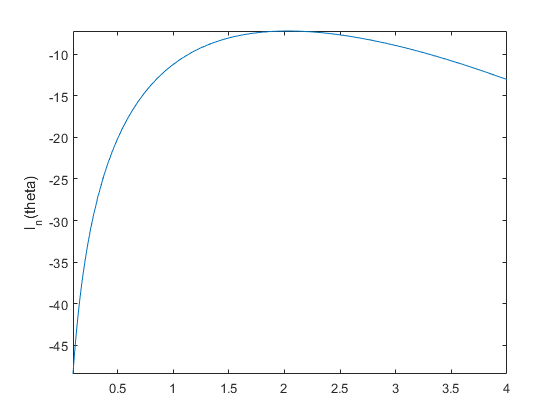
\includegraphics[width=0.5\textwidth]{q7n10.png}
\caption{Graph of $l_{10}(\theta)$ }
\end{figure}

n=30, $\hat{\theta}=2.1951$, sample: 1.3649	0.4220	0.2237	2.0550	0.4454	1.3580	0.8354	0.5516	1.5958	1.5912	0.1122	1.9013	1.5481	1.0045	0.1925	0.6636	0.6681	1.1091	0.2839	0.2365	0.9139	1.4916	0.1703	1.5614	0.3198	0.6918	0.8983	0.2961	1.2681	1.5597

\begin{figure}[ht]
\centering
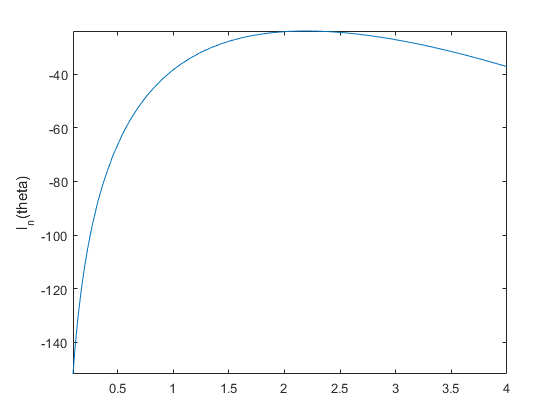
\includegraphics[width=0.5\textwidth]{q7n30.png}
\caption{Graph of $l_{30}(\theta)$ }
\end{figure}

n=50, $\hat{\theta}=2.2172$, sample: 2.4200	0.4695	0.2563	1.3419	0.1285	1.8532	0.9368	0.6773	0.2111	0.4122	0.2752	0.2789	0.4093	0.2045	0.4856	0.5103	0.8816	0.9168	0.0541	2.1615	1.9660	0.7944	0.3991	1.1527	0.8449	1.2815	1.2779	1.0545	1.2046	0.8783	0.9467	0.3820	0.3832	0.5037	0.0366	0.3420	0.8310	2.6198	2.2452	0.2491	0.3665	0.6405	1.2485	1.3772	0.1907	0.2554	3.3497	1.1131	1.0043	1.2785

 

\begin{figure}[ht]
\centering
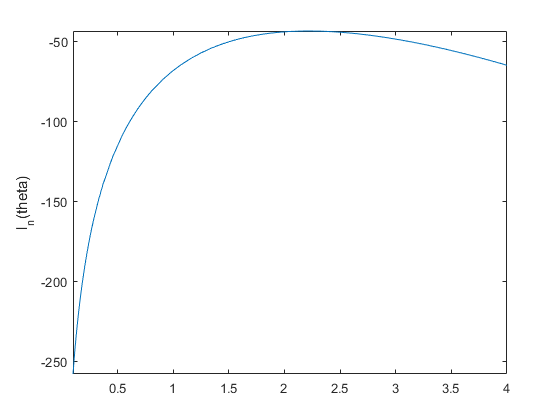
\includegraphics[width=0.5\textwidth]{q7n50.png}
\caption{Graph of $l_{50}(\theta)$ }
\end{figure}

\vspace{5mm}

As in question 3, we get very little difference in the shape of the graph as n is changed, since again can write $l_n(\theta)\approx n(2\ln\theta + \ln\frac{2}{\theta_0} -\theta\frac{2}{\theta_0})$ by taking expectations, which becomes a better estimate as n grows. We get a similarly shaped graph to question 3 too, since $f(x)=\ln x -x$ satisfies $f(x)\approx f(1/x)$ for small x. The peak is in a different position, and we see as n increases $\hat{\theta_n}$ approaches $\theta_0$ as before.

\newpage

\subsection*{Question 8}
The script $q8.m$ performs the required task. We get

\begin{figure}[ht]
\begin{minipage}[b]{0.5\linewidth}
\centering
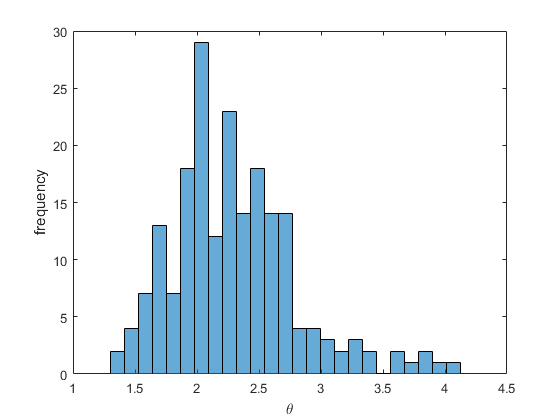
\includegraphics[width=\textwidth]{q8n10.png}
\caption{histogram of $\hat{\theta_{10}}(1)...\hat{\theta_{10}}(200)$}
\end{minipage}
\hspace{0.5cm}
\begin{minipage}[b]{0.5\linewidth}
\centering
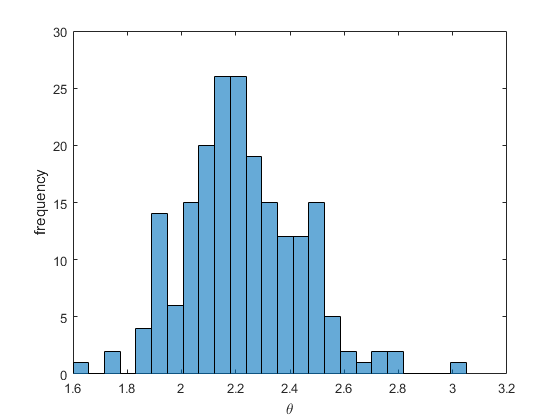
\includegraphics[width=\textwidth]{q8n50.png}
\caption{histogram of $\hat{\theta_{50}}(1)...\hat{\theta_{50}}(200)$}
\end{minipage}
\end{figure}

We see that the histogram peaks around $\theta_0=2.2$ for both, but the variance from this mean is smaller in the n=50 case than the n=10 case, as expected intuitively since more data is likely to make conclusions more accurate. Note if $X_1,X_2,...,X_N \sim \Gamma(2,\theta)$ then writing $X_i=Y_i^1+Y_i^2$ where $Y_i^j\sim Exp(\theta)$ independently, by induction using the argument of question 4, we get $\sum X_i \sim \Gamma(2N,\theta)$, and thus $\hat{\theta_n}=\frac{2n}{\sum{x_i}}$ follows an "inverse gamma distribution"\footnote{See \url{https://en.wikipedia.org/wiki/Inverse-gamma_distribution}}, which we can check has smaller variance for N large.



\subsection*{Question 9}
We have the probability density function $f(\phi,v)=\frac{1}{4\pi}e^{-v/2}$ and the transformation 

\begin{align*}
X &= \mu_1 +\sigma\sqrt{V}\cos\Phi\\
Y &= \mu_2 +\sigma\sqrt{V}\sin\Phi\\
\end{align*}

giving the Jacobian 

\begin{align*}
\left|\frac{\partial(X,Y)}{
\partial(V,\Phi)}\right|
=
\begin{vmatrix}
\partial X/\partial V & \partial X/\partial \Phi\\
\partial Y/\partial V & \partial Y/\partial \Phi\\
\end{vmatrix}
=
\begin{vmatrix}
 \sigma\cos\Phi/2\sqrt{V} & -\sigma\sqrt{V}sin\Phi\\
 \sigma\sin\Phi/2\sqrt{V} & -\sigma\sqrt{V}\cos\Phi\\
\end{vmatrix}
=\sigma^2/2
\end{align*}

and thus 

\begin{align*}
g(x,y)&=f(\phi(x,y),v(x,y))\left|\frac{\partial(V,\Phi)}{
\partial(X,Y)}\right|\\
&=\frac{1}{2\pi\sigma^2}e^{-\frac{1}{2\sigma^2}(x-\mu_1)^2+(y-\mu_2)^2}\\
&=\frac{1}{\sqrt{2\pi\sigma^2}}e^{-\frac{1}{2\sigma^2}(x-\mu_1)^2}\frac{1}{\sqrt{2\pi\sigma^2}}e^{-\frac{1}{2\sigma^2}(y-\mu_1)^2}
\end{align*}

so have $X \sim N(\mu_1,\sigma^2)$ and $Y \sim N(\mu_2,\sigma^2)$ independent by the factorisation criteria.

\subsection*{Question 10}
The function $generatenormal(\mu,\sigma,n)$ returns a random sample of size n from any given normal distribution. 

To generate an 80\% confidence interval, observe that if $X \sim N(\mu,1)$ then $Z=\sqrt{n}(\bar{X}-\mu) \sim N(0,1)$. Then for $z=\Phi^{-1}(0.9)$ have

\begin{equation*}
\mathbb{P}(-z<Z<z)=0.8
\quad\Leftrightarrow\quad \mathbb{P}(\bar{X}-\frac{z}{\sqrt{n}}<\mu<\bar{X}+\frac{z}{\sqrt{n}})=0.8\\
\end{equation*}
\begin{equation*}
\Leftrightarrow (\bar{X}-\frac{z}{\sqrt{n}},\bar{X}+\frac{z}{\sqrt{n}}) \quad \text{is an 80\% confidence set for $\mu$}
\end{equation*}

\subsection*{Question 11}

\begin{table}[ht]
\centering
\begin{tabular}{|l|l|l|l|}
\hline
$\bar{X}$   & lower bound  & upper bound  & contains 0?\\ \hline
0.046  & -0.082 & 0.174  & 1        \\ \hline
-0.148 & -0.276 & -0.020 & 0        \\ \hline
-0.055 & -0.183 & 0.073  & 1        \\ \hline
-0.039 & -0.167 & 0.089  & 1        \\ \hline
0.069  & -0.059 & 0.197  & 1        \\ \hline
-0.041 & -0.169 & 0.087  & 1        \\ \hline
-0.141 & -0.269 & -0.013 & 0        \\ \hline
0.091  & -0.037 & 0.219  & 1        \\ \hline
-0.121 & -0.250 & 0.007  & 1        \\ \hline
-0.219 & -0.347 & -0.091 & 0        \\ \hline
0.074  & -0.054 & 0.202  & 1        \\ \hline
0.086  & -0.042 & 0.215  & 1        \\ \hline
-0.054 & -0.182 & 0.075  & 1        \\ \hline
-0.113 & -0.241 & 0.016  & 1        \\ \hline
-0.133 & -0.261 & -0.005 & 0        \\ \hline
0.064  & -0.064 & 0.192  & 1        \\ \hline
0.105  & -0.023 & 0.233  & 1        \\ \hline
0.020  & -0.108 & 0.148  & 1        \\ \hline
-0.126 & -0.254 & 0.002  & 1        \\ \hline
-0.163 & -0.291 & -0.035 & 0        \\ \hline
0.036  & -0.092 & 0.164  & 1        \\ \hline
-0.009 & -0.137 & 0.119  & 1        \\ \hline
0.040  & -0.088 & 0.168  & 1        \\ \hline
-0.061 & -0.189 & 0.067  & 1        \\ \hline
0.048  & -0.080 & 0.177  & 1        \\ \hline
\end{tabular}
\caption{Results of 25 symmetric 80\% confidence intervals taken from samples of size 100 with mean 0 and variance 1, generated by $q11.m$}
\end{table}

Here we have 20 intervals containing the actual mean 0, and 5 not, as expected. By definition of the confidence interval, it is an interval with probability 0.8 of containing the mean, and since each sample is independent, the distribution of the T = the number of times the actual mean is in an 80\% confidence interval is $T\sim B(0.8,25)$ with $\mathbb{E}(T)=0.8\times 25=20$.

\subsection*{Question 12}

From the discussion above for $n=50,\mu=4$, the distribution of T is still $T\sim B(0.8,25)$ so we expect 20 to contain $\mu=4$ and 5 to not. Decreasing n will however increase the width of the interval to compensate.

\subsection*{Question 13}
By definition, for $Z_i$ independent standard normal distributions, $Q=\sum_{i=1}^k Z_i$ has the $\chi_k^2$ distribution, so to sample from a $\chi_k^2$ we can take k standard normal samples and sum their squares. The program $q13.m$ performs the required task, and overlays the scaled appropriate chi square pdf to confirm our program works as intended.\par
\vspace{5mm}

We see as n increases the histogram matches the shape of the pdf more closely, as expected. As k is increased, the histogram shifts right, since the mean of a $\chi_k^2$ variable is k. The histogram is also stretched, since the variance of a $\chi_k^2$ variable is 2k.\footnote{standard results, quoted from \url{https://en.wikipedia.org/wiki/Chi-squared_distribution}}


\begin{figure}[h]
\begin{minipage}[b]{0.5\linewidth}
\centering
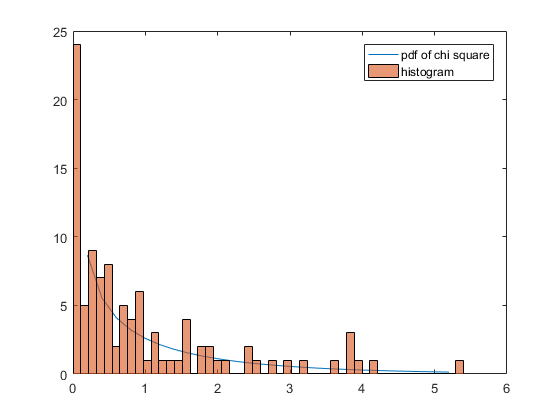
\includegraphics[width=\textwidth]{k1n100.png}
\caption{k=1 n=100}
\end{minipage}
\hspace{0.5cm}
\begin{minipage}[b]{0.5\linewidth}
\centering
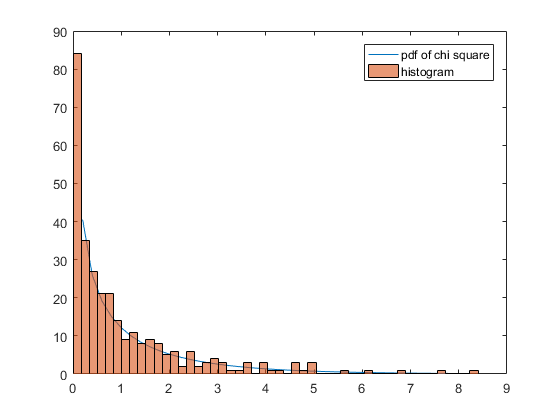
\includegraphics[width=\textwidth]{k1n300.png}
\caption{k=1 n=300}
\end{minipage}
\end{figure}
	

\begin{figure}[ht]
\begin{minipage}[b]{0.5\linewidth}
\centering
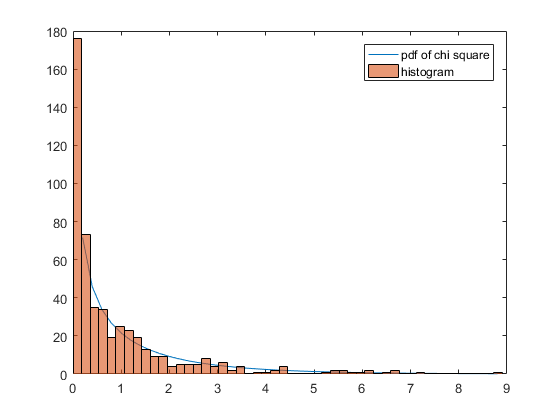
\includegraphics[width=\textwidth]{k1n500.png}
\caption{k=1 n=500}
\end{minipage}
\hspace{0.5cm}
\begin{minipage}[b]{0.5\linewidth}
\centering
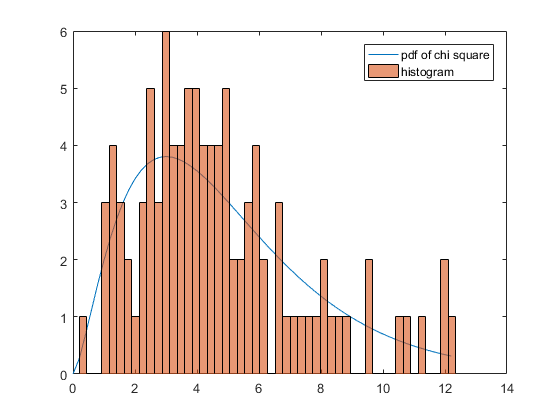
\includegraphics[width=\textwidth]{k5n100.png}
\caption{k=5 n=100}
\end{minipage}
\end{figure}

\begin{figure}[ht]
\begin{minipage}[b]{0.5\linewidth}
\centering
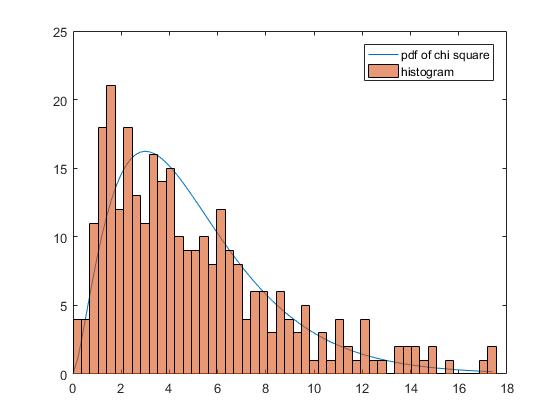
\includegraphics[width=\textwidth]{k5n300.png}
\caption{k=5 n=300}
\end{minipage}
\hspace{0.5cm}
\begin{minipage}[b]{0.5\linewidth}
\centering
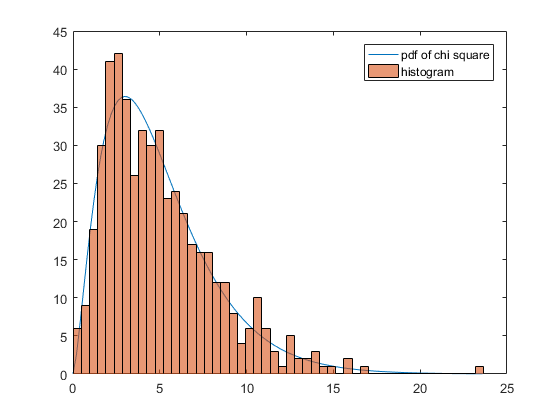
\includegraphics[width=\textwidth]{k5n500.png}
\caption{k=5 n=500}
\end{minipage}
\end{figure}

\begin{figure}[ht]
\begin{minipage}[b]{0.5\linewidth}
\centering
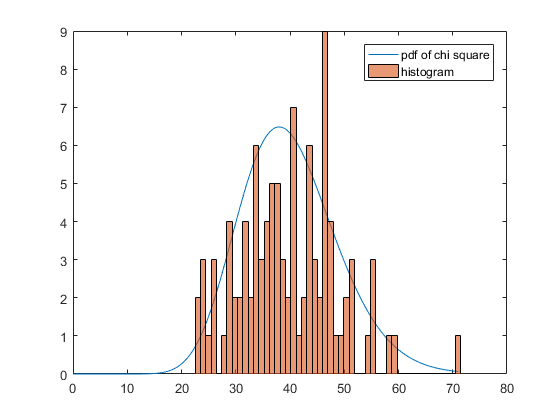
\includegraphics[width=\textwidth]{k40n100.png}
\caption{k=40 n=100}
\end{minipage}
\hspace{0.5cm}
\begin{minipage}[b]{0.5\linewidth}
\centering
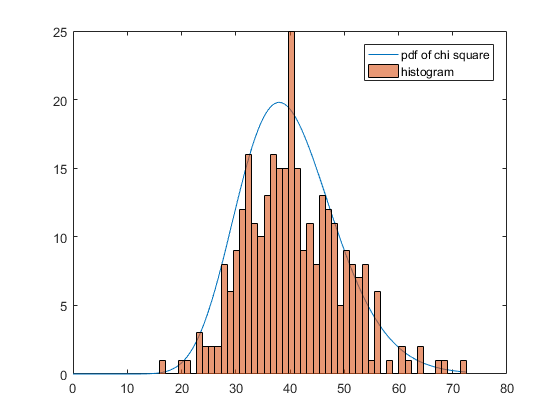
\includegraphics[width=\textwidth]{k40n300.png}
\caption{k=40 n=300}
\end{minipage}
\end{figure}

\begin{figure}[ht]
\centering
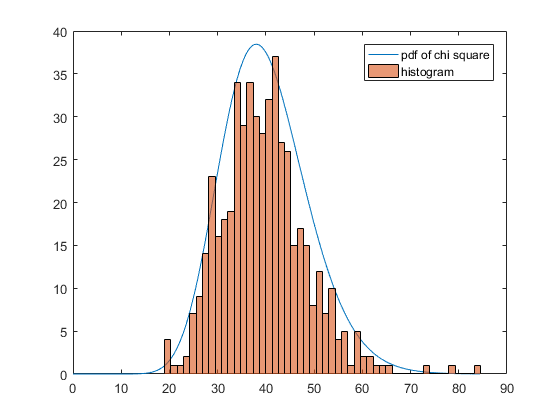
\includegraphics[width=0.5\textwidth]{k40n500.png}
\caption{k=40 n=500}
\end{figure}




\clearpage

\subsection*{Programs}

\subsubsection*{The Exponential Distribution}

$q2.m$

\begin{verbatim}
n=1000
U=rand(n,1)
theta_0=1.2
X=-log(1-U)/(theta_0)

l=@(m) 0


for i=1:n
    
    li=@(m) log(log(2))-log(m)-log(2)*X(i)/m;
    l=@(m) l(m)+li(m);  
end

fplot(l,[0.1,1])
%hold on
%line([sum(X)*log(2)/n sum(X)*log(2)/n],[-10 0],'LineWidth',1)
xlabel('m')
ylabel('l_n(m)')

m=log(2)/theta_0
mhat=sum(X)*log(2)/n
\end{verbatim}

\vspace{5mm}

$q7.m$

\begin{verbatim}
n=50
U=rand(n,1)
V=rand(n,1)
theta_0=2.2
X=-log(1-U)/theta_0
Y=-log(1-V)/theta_0
Z=X+Y

l=@(m) 0


for i=1:n
    
    li=@(theta) 2*log(theta)+log(Z(i))-theta*Z(i);
    l=@(theta) l(theta)+li(theta);  
end

fplot(l,[0.1,4])
hold on
%line([sum(X)*log(2)/n sum(X)*log(2)/n],[-10 0],'LineWidth',1)
ylabel('l_n(theta)')

thetahat=2*n/sum(Z)
	
\end{verbatim}

\vspace{5mm}

$q8.m$

\begin{verbatim}

n=100
N=200
theta_0=2.2

for i=1:N
U=rand(n,1)
V=rand(n,1)
X=-log(1-U)/theta_0
Y=-log(1-V)/theta_0
Z=X+Y
thetahat(i)=2*n/sum(Z)
end

histogram(thetahat,25)
xlabel('\theta')
ylabel('frequency')

\end{verbatim}

\subsubsection*{The Normal Distribution}

$generatenormal.m$

\begin{verbatim}
function [ X ] = generatenormal( mu,sigma,n )

for i = 1:n
    
    A=rand;
    B=rand;
    phi=2*pi*A;
    V=-2*log(1-B);
    X(i)=mu+sigma*sqrt(V)*cos(phi);
    
end

end
\end{verbatim}

\vspace{5mm}

$q11.m$

\begin{verbatim}
n=50
z=norminv(0.9)
mu=4
for j = 1:25   
    X=generatenormal(mu,1,n)
    Xbar(j)=sum(X)/n
    upper(j)=Xbar(j)+z/sqrt(n)
    lower(j)=Xbar(j)-z/sqrt(n)
    if mu <=upper(j) & mu>=lower(j)
        contains(j)=1
    else
        contains(j)=0
    end
end

count=0
for i=1:25
    if contains(i)==1
        count=count+1
    end
end
\end{verbatim}

\subsubsection*{The $\chi^2$ Distribution}

$q13.m$

\begin{verbatim}
k=40
n=500
chi=[]
for i=1:n
X=generatenormal(0,1,k);
chi(i)=sum(X.^2);
end

x = 0:0.2:max(chi);
y = n*max(chi)/50*chi2pdf(x,k);  
plot(x,y)
hold on
histogram(chi,50) 
legend('pdf of chi square', 'histogram')
    
%normalise needs area - only approx
\end{verbatim}

        
        

\end{document}


